\documentclass[11pt]{beamer}
\usetheme{Frankfurt}
\usecolortheme{crane}
\usepackage[utf8]{inputenc}
\usepackage[english]{babel}
\usepackage{amsmath}
\usepackage{amsfonts}
\usepackage{amssymb}
\usepackage{graphicx}
\usepackage{fancyvrb}
%\usepackage{circuitikz}
\author{Maximilian Heim}
\title{Return Oriented Programming}
%\setbeamercovered{transparent} 
%\setbeamertemplate{navigation symbols}{} 
\logo{
\includegraphics[width=0.1\textwidth]{logo.png}}
\institute{University Albstadt-Sigmaringen} 
\date{\today} 
\subject{Offensive Security Methods}
\begin{document}

\begin{frame}
\titlepage
\end{frame}

\begin{frame}
\tableofcontents
\end{frame}

\section{Introduction}
\subsection{Return Oriented Programming}
\begin{frame}
    \frametitle{What is Return Oriented Programming?}
    \begin{itemize}
    \item A type attack that exploits buffer overruns
    \item Published by Hovav Shacham in 2007
    \item Arised as a technique to counter security mechanisms (NX)
    \item Big binary $\rightarrow$ ROP is turing complete
    \item Many authors refer to ret-to-libc as ROP
    \end{itemize}
\end{frame}

\section{How does it work?}
\begin{frame}
    \frametitle{Overview}
    \begin{enumerate}
        \item Search the binary for gadgets: return (0xC3) bytes that contain useful instructions before
        \item Generate a list of these gadgets, called ROP chain
        \item Generate a payload with the addresses of these gadgets
        \item Insert payload via buffer overrun
    \end{enumerate}
\end{frame}
\begin{frame}
    \frametitle{ROP gadgets}
    \begin{itemize}
        \item Gadgets are machine instructions that end on a return
        \item Tools: ROPgadget (\url{https://github.com/JonathanSalwan/ROPgadget}), ropper (\url{https://github.com/sashs/Ropper}), Radare2, pwntools....
    \end{itemize}
    \begin{figure}[h]
        \caption{ROP Gadgets}
        \centering
        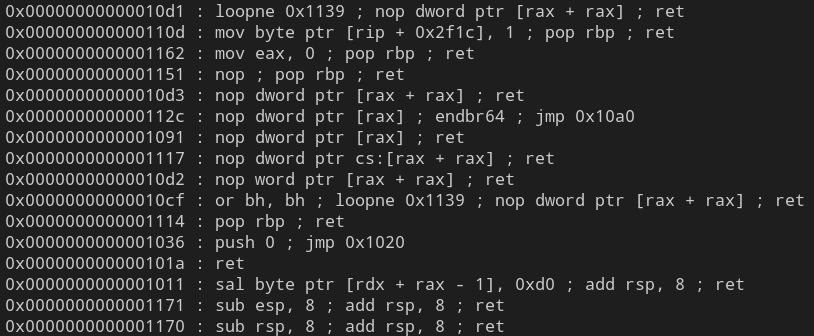
\includegraphics[width=0.8\textwidth]{gadget.png}\label{gadget}
    \end{figure}

\end{frame}

\begin{frame}[fragile]
    \frametitle{Useful gadgets: Write to register}
    \begin{itemize}
        \item Especially useful are pop instructions
    \end{itemize}
    \begin{Verbatim}
        POP eax, ret;
    \end{Verbatim}
    \begin{itemize}
        \item These allow us to write arbitrary values into registers
        \item However, sometimes we do not find a pop into our desired register (e.g. r14), here we can improvise and use something like
    \end{itemize}
    \begin{Verbatim}
        xor r14, r14
        pop r12
        xor r14, r12
    \end{Verbatim}
\end{frame}

\begin{frame}
    \frametitle{References}
    \url{https://trustfoundry.net/basic-rop-techniques-and-tricks/}
    
\end{frame}


\end{document}